\documentclass[10pt,a4paper]{report}
\usepackage[utf8]{inputenc}
\usepackage[french]{babel}
\usepackage{graphicx}
\usepackage{float}

\begin{document}
\begin{center}
\begin{tabular*}{\textwidth}{l @{\extracolsep{\fill}} r}

  %\hline
  
\includegraphics [width=40mm]{ENSEIRB-MATMECA.ps} &
  %\adjustbox{valign=m}{
  \raisebox{0.75\height}
           {
\includegraphics [width=40mm]{logo-LaBRI-couleur.ps}}
           %}\\
           %\hline
           
\end{tabular*}

\vspace{\stretch{1}}
      
\textsc{\Huge Manuel d'utilisation de PFA-Nethack}\\[0.5cm]
\rule{0.4\textwidth}{1pt}
           
\vspace{\stretch{1}}
           
%{\huge \bfseries \reporttitle}\\[0.4cm]
%\HRule \\[1.5cm]

\begin{center}
  
  \begin{flushleft}
    \large
    \emph{Auteurs :}\\
    \begin{itemize}
    \item Benoît Ruelle
    \item David Bitonneau
    \item Ludovic Hofer
    \end{itemize}
  \end{flushleft}
  
  
  \begin{flushright}
    \large
    \emph{Responsables :}\\
    Pédagogique - M.~Renault\\
    Client - M.~Le Borgne\\
  \end{flushright}
\end{center}

\vspace{\stretch{1}}
                  
{\large Deuxième année, filière informatique}

~

{\large 16 octobre 2012 - 29 mars 2013}\\
                  
\end{center}
\thispagestyle{empty}
\pagebreak

\chapter{Utilisation du code fourni}
\section{Génération des exécutables}
TODO David/Benoit

\section{Lancer une partie avec un bot}
TODO

\section{Paramétrer l'exécution de nethack}
TODO

\section{Lancer plusieurs parties grâce à un script}
Le script \emph{game\_runner.sh} permet à l'utilisateur de lancer facilement
un grand nombre de parties qui ne diffèrent que par la graine aléatoire
utilisée.
\\
Il est possible de lancer plusieurs instances de ce script en simultané, et ce
même si elles enregistrent leurs résultats dans la même base de donnée. Chaque
script créé un dossier dans /tmp/ avant d'y copier le code de nethack ainsi que
le bot, ceci permet de continuer à travailler sur les bots ou sur le code de
nethack sans risquer d'interférer avec les parties déjà lancées. Si ce
comportement n'est pas souhaité, il est relativement simple de commenter la
partie du code qui y est associé.
\\
Plusieurs options peuvent être utilisées pour ce script, il est possible
d'obtenir plus de détails facilement en utilisant la commande suivante :
\emph{game\_runner.sh -h}.

\section{Remplir une base de donnée}
Le script \emph{data\_builder.sh} permet de générer facilement une base de
données contenant les résultats d'un grand nombre de parties. Ce script n'est
pas paramétré, mais il est aisément modifiable à la main, son but est
principalement de fournir une base pour permettre à un utilisateur novice
d'ajouter ou de supprimer des bots où des nombres de mouvements autorisés à
l'ensemble des parties à lancer.
\\
Bien que lui même ne lance pas plusieurs processus, ce script peut
parfaitement être exécuté $N$ fois, $N$ étant le nombre de processeur
disponible. Cependant l'affichage n'a pas été prévu pour gérer plusieurs
processus à l'aide d'un seul terminal, ainsi, si l'on souhaite observer
l'évolution des exécutions, il est conseillé des les exécuter dans $N$
terminaux différents.

\section{Revoir une partie}
TODO Benoit

\section{Générer des graphiques}
Afin de jauger les performances des différents bots, mais aussi afin de
déceler des bugs, il peut être pratique de générer des graphiques illustrant les
données qui ont été générées par les parties jouées. Ces graphiques peuvent
non seulement permettre d'évaluer la répartition des résultats d'un bot,
mais aussi de comparer les performances moyennes des bots entre eux. Il existe
un dernier type de graphe qui permet de jauger la répartition des portes
secrètes et des couloirs secrets en fonction de la position dans la carte.

\subsection{Graphiques analysant un bot}
Le script \emph{impulse\_graph.sh} permet de créer un grand nombre de
graphiques indiquant la répartition des performances du bot, ces graphiques
sont générés à l'aide de gnuplot et se présentent sous cette forme.

\begin{figure}[H]
  \center{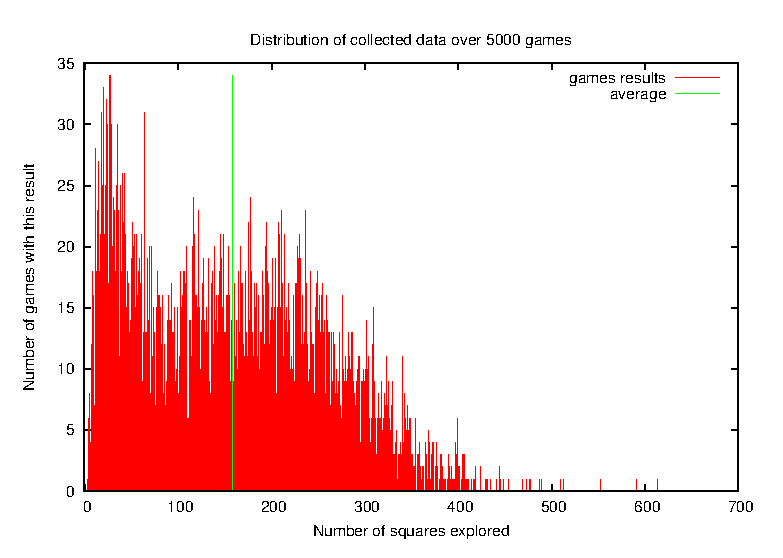
\includegraphics[width=\textwidth]{impulse_graph.eps}}
	\caption{\label{fig:impulse_graph} Un exemple de fichier produit par impulse\_graph.sh}
\end{figure}

Lors de son exécution, ce script créé un dossier présent par bot trouvé dans
la base de donnée passée en paramètre et y ajoute tous les graphiques le
concernant. En conséquence, il est hautement recommandé que le dossier ne
contienne que la base de donnée lorsque celui-ci est exécuté.

\subsection{Graphiques comparant des bots}
Afin de comparer les performances des bots dans différents domaines, il est
possible d'utiliser le script \emph{move\_graph.sh}. Celui-ci génère des
graphiques pour les principales performances générées par les bots, les
résultats se présentent sous cette forme.

\begin{figure}[H]
  \center{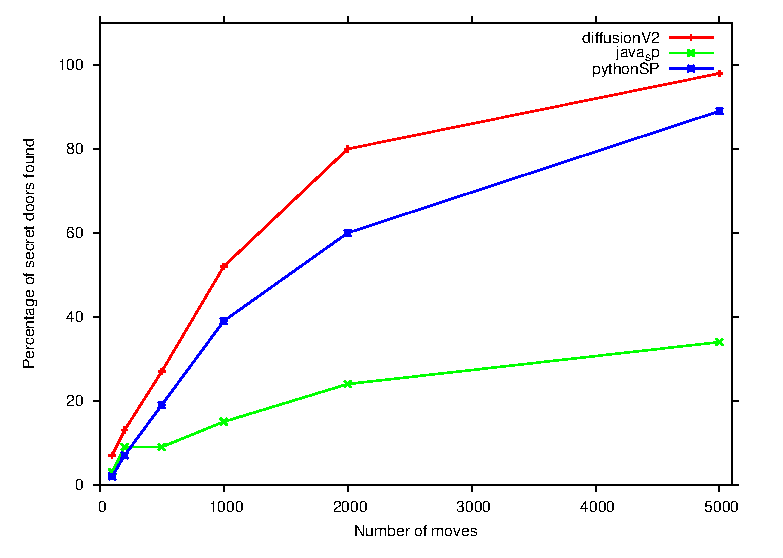
\includegraphics[width=\textwidth]{move_graph.eps}}
  \caption{\label{fig:move_graph} Un exemple de fichier produit par move\_graph.sh}
\end{figure}

\subsection{Graphiques indiquant la répartition de différents objets}
Afin d'évaluer la répartition des portes secrètes ou des couloirs secrets,
quatres scripts sont mis à dispositions :

\begin{itemize}
\item 2d\_doors\_graph.sh
\item 3d\_doors\_graph.sh
\item 2d\_scorrs\_graph.sh
\item 3d\_scorrs\_graph.sh
\end{itemize}

Les scripts \emph{2d} produisent un graphique indiquant le nombre de cases
correspondant à la catégorie demandée sur chaque ligne et un autre par rapport
aux colonnes. 

\begin{figure}[H]
  \center{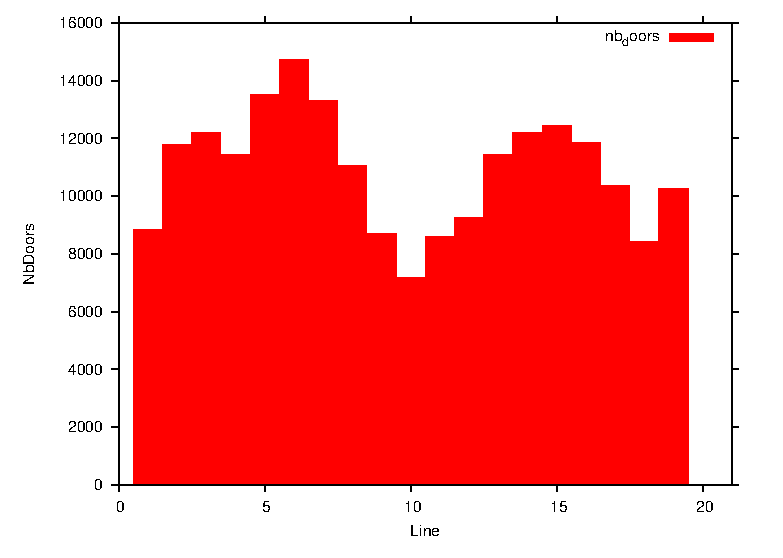
\includegraphics[width=\textwidth]{2d_graph.eps}}
  \caption{\label{fig:2d_graph} Un exemple de graphique 2d}
\end{figure}


Les scripts \emph{3d} ne produisent pas de fichiers, mais ils ouvrent une
fenêtre gnuplot permettant de visualiser un graphe indiquant le nombre de cases
de la catégorie demandée pour chaque position. 

\begin{figure}[H]
  \center{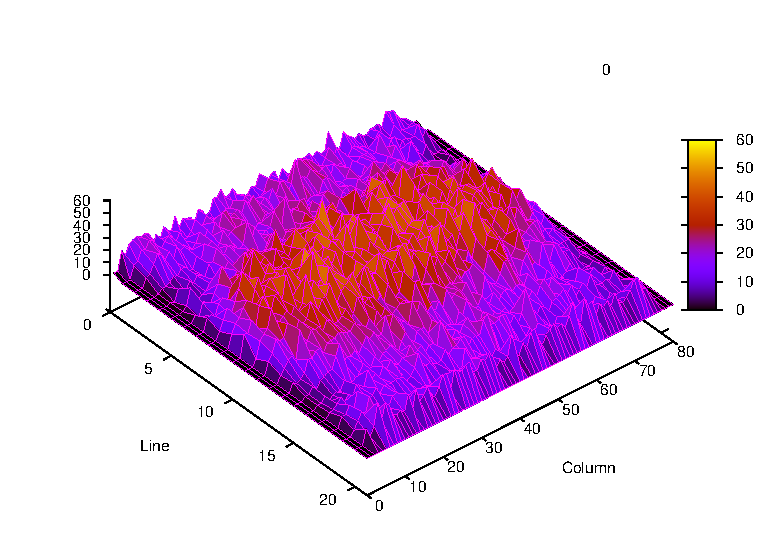
\includegraphics[width=\textwidth]{3d_graph.eps}}
  \caption{\label{fig:3d_graph} Un exemple de visualisation en 3d}
\end{figure}

\chapter{Les bots}
\section{Le starter package java}
Afin de pouvoir rapidement commencer à coder des bots, un \emph{starter package}
en java est fourni, les fonctionnalités fournies sont principalement la lecture
de la carte et la vérification de la validité des mouvements.
\\
Ce bot se contente de lister les actions possibles et d'en choisir une de façon
aléatoire, avec tout de même certaines actions prioritaires. Cette base permet
de pouvoir tester différentes stratégie sans avoir à implémenter à nouveau la
réception et l'envoi de message aux bots.

\section{Le bot diffusion}
Le principe de ce bot est d'établir des scores pour chaque cases et de diffuser
ensuite les valeurs à tous les voisins, ainsi la principale différence avec les
autres bots est que la complexité est bien plus élevée étant donnée que pour
choisir la prochaine action, il n'y a pas que le voisinage immédiat qui est
observé. Ce surcoût de temps permet en revanche d'avoir des meilleurs résultats
et la possibilité de modifier les scores facilement permet de changer les
objectifs en changeant uniquement des constantes.
\\
Une fois tous les scores calculés et la diffusion effectuée, l'action choisie
est celle ayant le score le plus élevé parmi celles qui sont autorisées. Ce bot
est donc totalement déterministe. Quelques attentions ont été portées à
l'optimisation afin de réduire légèrement le temps d'exécution, cependant, il
est certainement possible d'améliorer encore grandement les performances en
optimisant certaines parties du code.

\section{Le starter package python}
TODO Benoît

\section{Le bot spécialisé}
TODO David

\chapter{Description technique}
\section{Les patchs du noyau de nethack}

\subsection{Les patchs nécessaires}
TODO hook etc

\subsection{Les patchs facultatifs}
TODO mode de jeu etc (cf doc de spec)

\section{Stockage des résultats}
Les résultats des parties sont stockés dans une base de données afin de ne pas perdre
trop d'informations et de pouvoir effectuer toute sorte de traitements dessus. Une vue
fournissant certains détails supplémentaires \footnote{Nombre de portes secrètes,
nombre de portes secrètes trouvées, nombre de couloirs secrets et nombre de couloirs
secrets trouvés.} est aussi disponible afin de faciliter l'utilisation de celle-ci.

\begin{figure}[H]
  \center{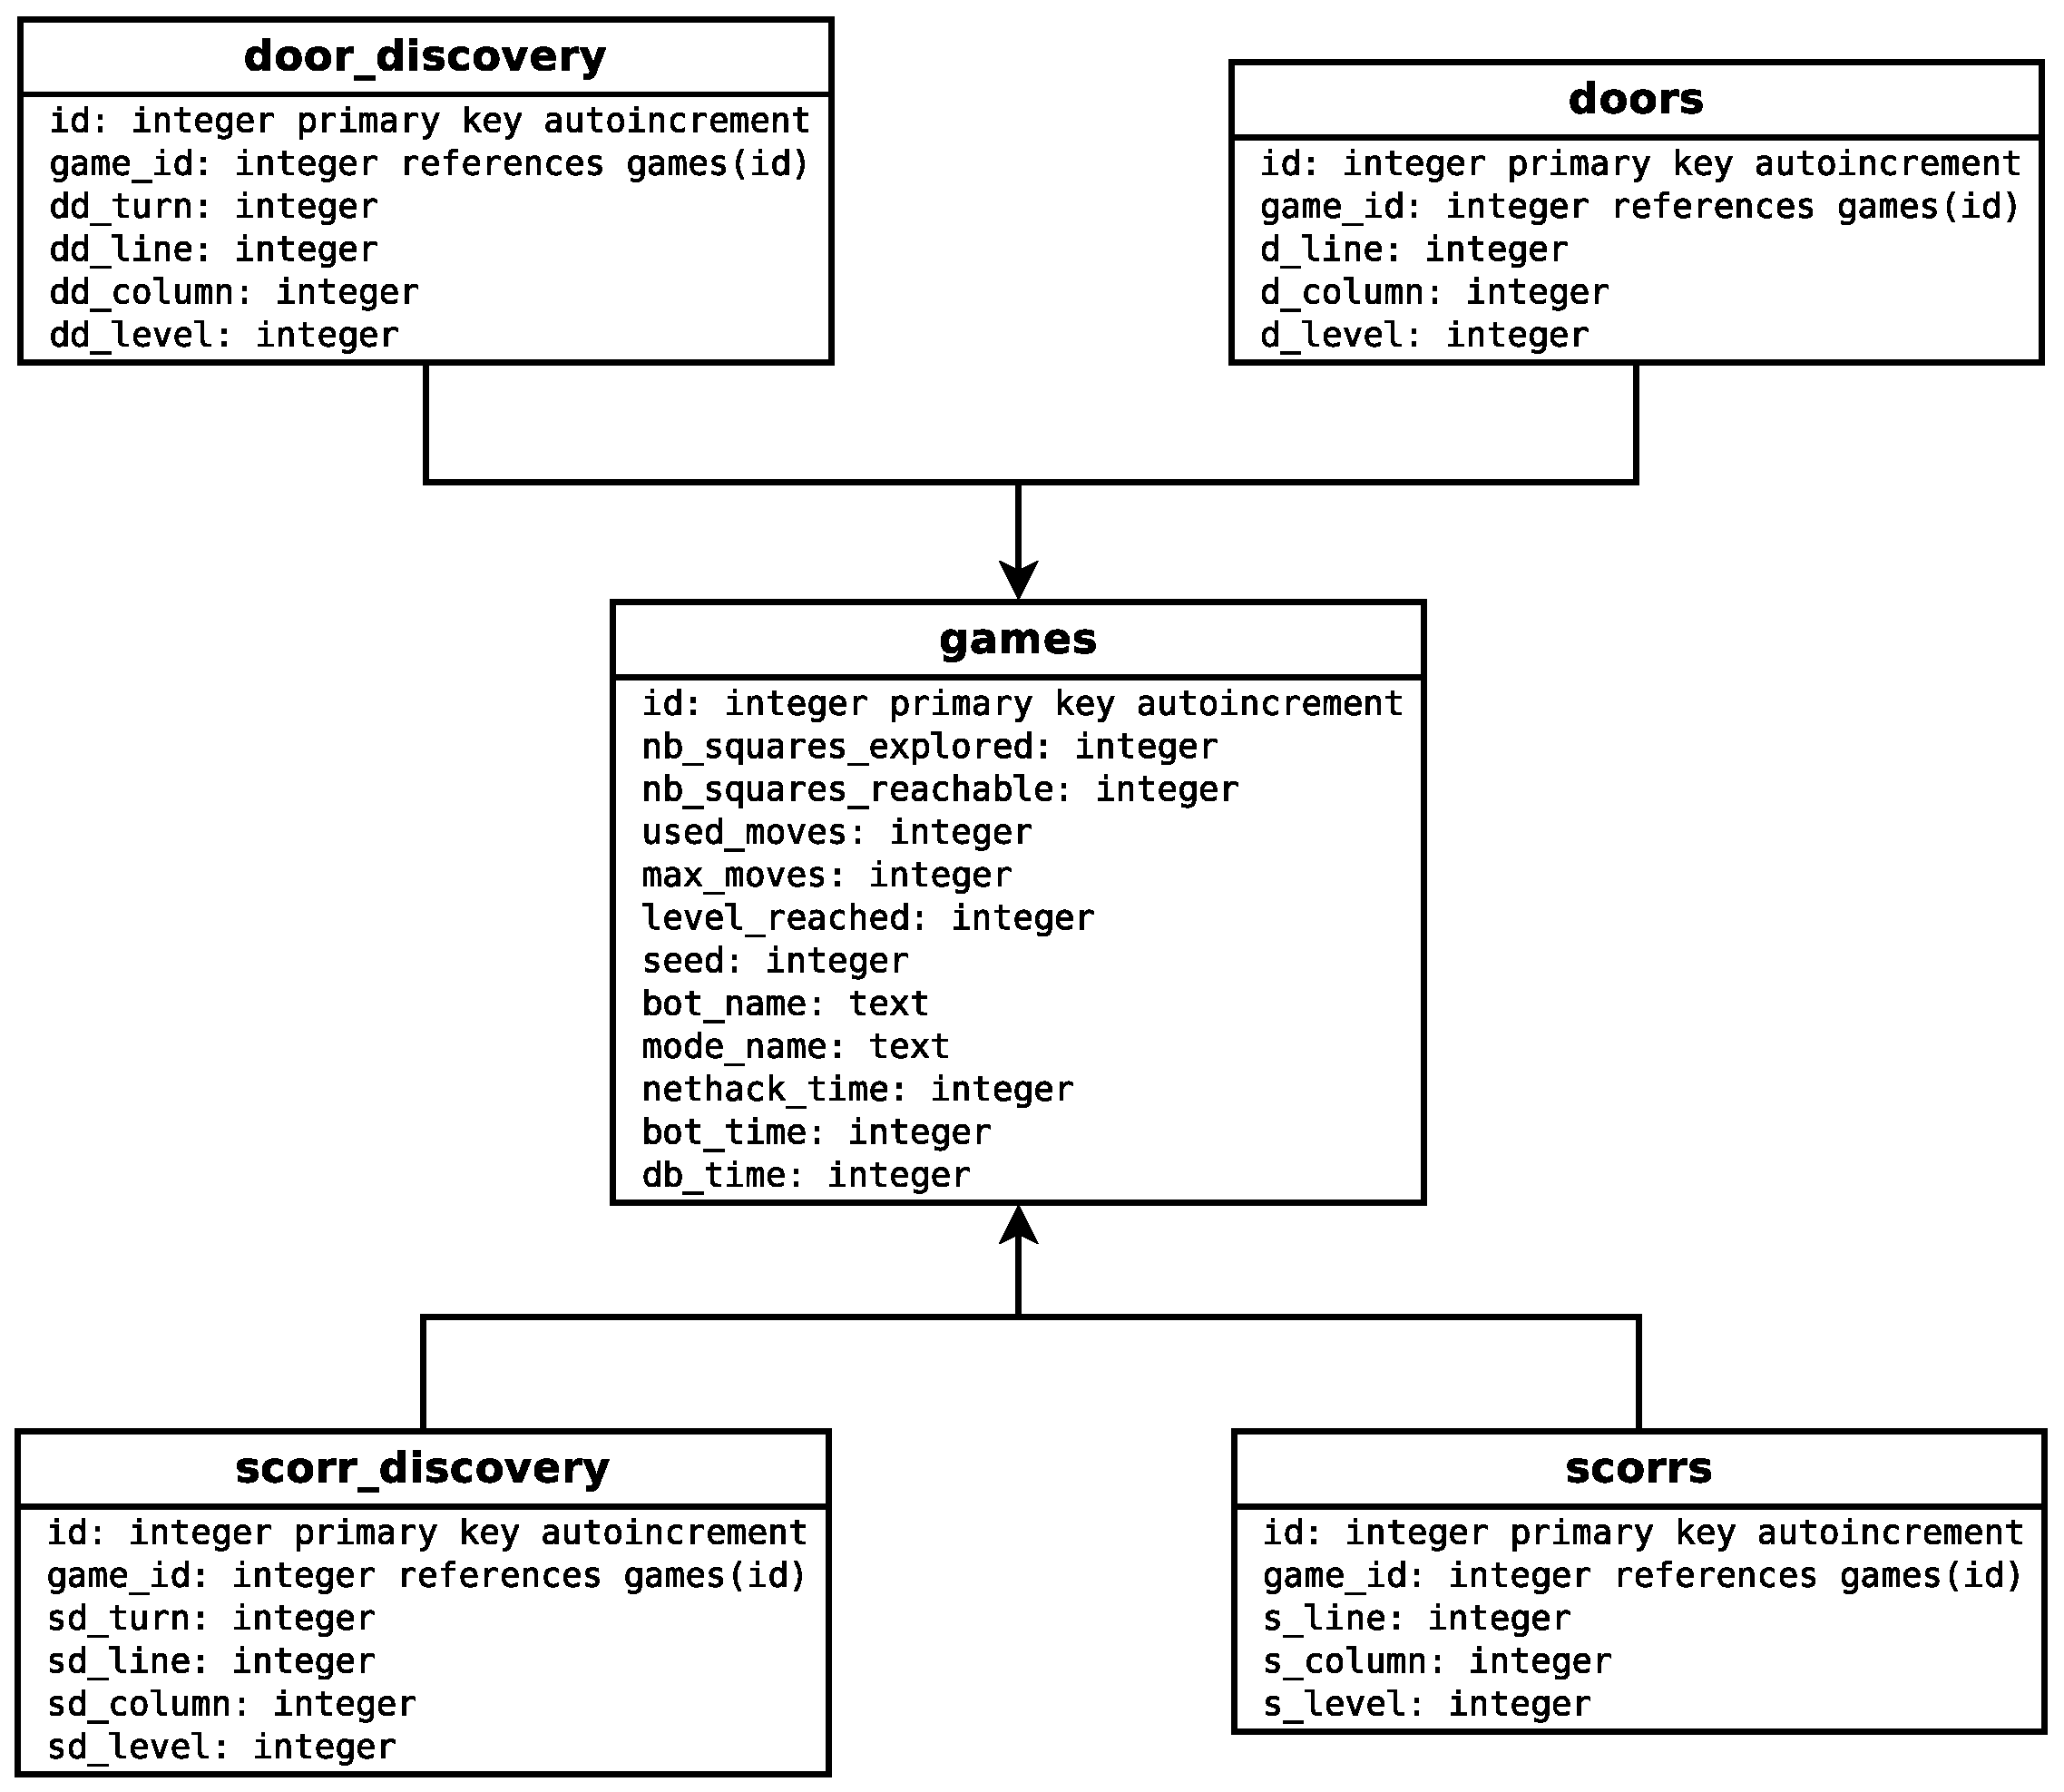
\includegraphics[width=\textwidth]{../../database_details/schema.eps}}
	\caption{\label{fig:database} Schéma de la base de données}
\end{figure}

\chapter{Apporter ses propres modifications au code existant}
\section{Modifier du code source contenu dans les hooks}
Il est aisé de modifier du code source à l'intérieur des différents hooks
fournis car le script \emph{nh-setup.sh} permet de recompiler l'exécutable
nethack en recompilant tous les fichiers sources nécessaires. Ainsi, il n'y aura
pas de modifications plus profonde à faire dans ce cas là. Cependant, si un
nouveau fichier est utilisé, il faudra néanmoins modifier le Makefile présent
dans le dossier \emph{install/nh/src} afin que les dépendances soient prises en
compte. Comme le fichier Makefile n'est pas recopié par défaut vers sa
destination, il faudra aussi spécifier à nethack que l'on ne souhaite pas
réutiliser le code existant (ou copier le Makefile avant afin de gagner du temps
de compilation).

\section{Modifier les données stockées}

\section{Ajouter de nouveau patchs}


\chapter{Dysfonctionnements connus}
\section{Sémaphore bloquée de façon permanente}
Lorsqu'un utilisateur tue un processus de nethack, le processus peut se terminer
alors qu'il est dans une zone critique, il ne libère donc pas l'accès à la base
de données, une solution peut être implémentée à l'aide d'un gestionnaire de
signal, cependant au vu des appels à une bibliothèque externe, il est possible
que cela ne suffise pas. Actuellement, la meilleure solution dans ce cas est
d'effacer la sémaphore afin que les nouveaux processus de nethack ne soient pas
bloqués lorsqu'ils tentent d'écrire dans la base de données. Sur certains
systèmes, les fichiers de sémaphore nommées peuvent être trouvés dans 
\emph{/dev/shm/}, dans le cas où l'utilisateur ne parvient pas à trouver
comment effacer les sémaphore nommées, il existe deux autres solutions :
renommer la base de données afin de changer le nom de sémaphore associé ou
redémarrer \footnote{attention, si la base de données est dans les fichiers
temporaires, il est 
conseillé de la déplacer avant}.

\end{document}
